\section{Tracer un exemple}
\q{Ecrire une procédure }\il{lignes(n, k0, k1)}\q{qui dessine les lignes de
  niveau de $f(x, y) = x^2+2y^2+2xy=k$ pour $k$ allant de }\il{k0}\q{ à }\il{k1}
\q{en recherchant les départs de la ligne de niveau sur la droite $y = x$ du
  plan.}

En supprimant la ligne \il{plt.show()} de la fonction \il{traceLinge()}:
\codeFromFileT{main.py}{section-07/qa.py}
Ce qui donne :
\begin{center}
  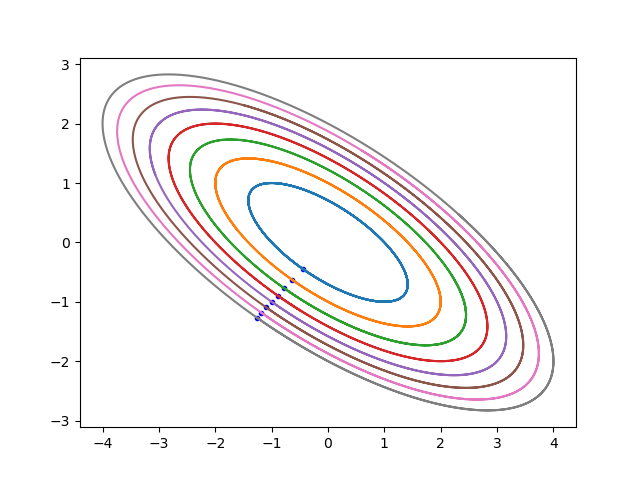
\includegraphics[scale=0.6]{section-07/qb.png}
\end{center}
